\documentclass[tikz,border=15pt]{standalone}
\usepackage{tikz}
\usepackage{amsmath}
\usetikzlibrary{arrows.meta,positioning,shapes}

\begin{document}
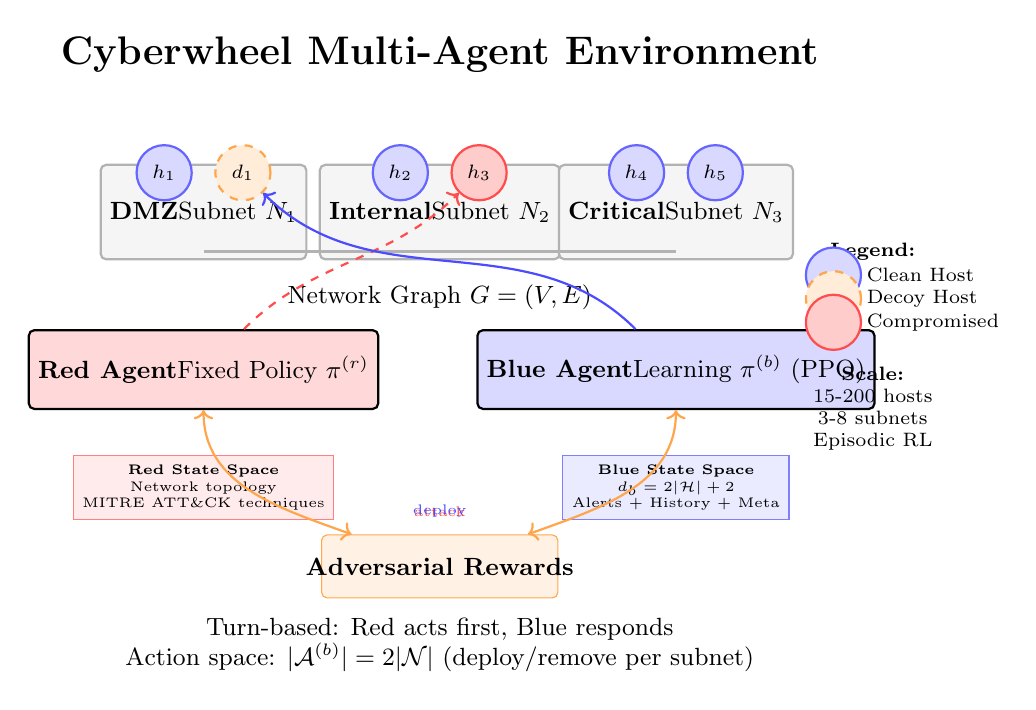
\begin{tikzpicture}[
    host/.style={circle, draw=blue!60, fill=blue!15, minimum size=7mm, font=\scriptsize, thick},
    decoy/.style={circle, draw=orange!70, fill=orange!15, minimum size=7mm, font=\scriptsize, thick, dashed},
    compromised/.style={circle, draw=red!70, fill=red!20, minimum size=7mm, font=\scriptsize, thick},
    subnet/.style={rectangle, draw=gray!60, fill=gray!8, minimum width=20mm, minimum height=12mm, font=\small, thick, rounded corners=2pt},
    agent/.style={rectangle, draw=black, fill=yellow!15, minimum width=22mm, minimum height=10mm, font=\small, thick, rounded corners=2pt}
]

% Title
\node[font=\Large\bfseries] at (0, 6) {Cyberwheel Multi-Agent Environment};

% Network subnets - well spaced
\node[subnet] (subnet1) at (-3, 4) {\textbf{DMZ}\\Subnet $N_1$};
\node[subnet] (subnet2) at (0, 4) {\textbf{Internal}\\Subnet $N_2$};  
\node[subnet] (subnet3) at (3, 4) {\textbf{Critical}\\Subnet $N_3$};

% Representative hosts - minimal set
\node[host] (h1) at (-3.5, 4.5) {$h_1$};
\node[decoy] (d1) at (-2.5, 4.5) {$d_1$};

\node[host] (h2) at (-0.5, 4.5) {$h_2$};
\node[compromised] (h3) at (0.5, 4.5) {$h_3$};

\node[host] (h4) at (2.5, 4.5) {$h_4$};
\node[host] (h5) at (3.5, 4.5) {$h_5$};

% Network backbone
\draw[thick, gray!60] (-3, 3.5) -- (0, 3.5) -- (3, 3.5);
\node[below, font=\small] at (0, 3.2) {Network Graph $G = (V,E)$};

% Agents - well separated vertically
\node[agent, fill=red!15] (red) at (-3, 2) {\textbf{Red Agent}\\Fixed Policy $\pi^{(r)}$};
\node[agent, fill=blue!15] (blue) at (3, 2) {\textbf{Blue Agent}\\Learning $\pi^{(b)}$ (PPO)};

% Key interactions - clean arrows
\draw[->, thick, red!70, dashed] (red) to[out=45, in=225] (h3) node[midway, above, font=\tiny] {attack};
\draw[->, thick, blue!70] (blue) to[out=135, in=315] (d1) node[midway, above, font=\tiny] {deploy};

% Essential state info - positioned to avoid overlap
\node[rectangle, draw=blue!50, fill=blue!8, font=\tiny, align=center, minimum width=20mm] at (3, 0.5) {
    \textbf{Blue State Space}\\
    $d_b = 2|\mathcal{H}| + 2$\\
    Alerts + History + Meta
};

\node[rectangle, draw=red!50, fill=red!8, font=\tiny, align=center, minimum width=20mm] at (-3, 0.5) {
    \textbf{Red State Space}\\
    Network topology\\
    MITRE ATT\&CK techniques
};

% Reward system - centered
\node[rectangle, draw=orange!70, fill=orange!10, minimum width=30mm, minimum height=8mm, rounded corners=2pt] at (0, -0.5) (reward) {};
\node[font=\small] at (reward.center) {\textbf{Adversarial Rewards}};

% Reward connections - clean
\draw[<->, orange!70, thick] (red) to[out=270, in=160] (reward);
\draw[<->, orange!70, thick] (blue) to[out=270, in=20] (reward);

% Key info - bottom
\node[font=\small, align=center] at (0, -1.5) {
    Turn-based: Red acts first, Blue responds\\
    Action space: $|\mathcal{A}^{(b)}| = 2|\mathcal{N}|$ (deploy/remove per subnet)
};

% Simple legend - right side
\node[font=\scriptsize] at (5.5, 3.5) {\textbf{Legend:}};
\node[host] at (5, 3.2) {};
\node[right, font=\scriptsize] at (5.3, 3.2) {Clean Host};
\node[decoy] at (5, 2.9) {};
\node[right, font=\scriptsize] at (5.3, 2.9) {Decoy Host};
\node[compromised] at (5, 2.6) {};
\node[right, font=\scriptsize] at (5.3, 2.6) {Compromised};

% Environment scale - right side bottom
\node[font=\scriptsize, align=center] at (5.5, 1.5) {
    \textbf{Scale:}\\
    15-200 hosts\\
    3-8 subnets\\
    Episodic RL
};

\end{tikzpicture}
\end{document}